\documentclass[nochap]{apuntes}

\usepackage{tikz}
\tikzset{>=latex}
\usetikzlibrary{decorations.pathmorphing,patterns}
\begin{document}

\subsection{Problemas lineales con coeficientes constantes}
\label{secEcHomoLinealConstante}
En el caso homogéneo, en el que tenemos una EDO

\[ y^{n)} + a_{n-1}y^{n-1)} + \dotsb + a_1y' + a_0 y = 0 \]

podemos obtener un polinomio característico \todo{Explicar de dónde sale. Matriz y eso}

\[ λ^n + a_{n-1}λ^{n-1} + \dotsb + a_1λ + a_0 = 0 \]

que, resolviéndolo, obtenemos las soluciones asociadas a cada una de las raíces. Podemos tener varias opciones en este caso. 

\begin{itemize}
\item Si $λ_0$ es una raíz simple, entonces una solución es $y_0(t) = e^{λ_0t}$.
\item Si $λ_1$ es una raíz con multiplicidad $k$, por el método de variación de las constantes encontraremos $k$ soluciones de la forma $t^ie^{λ_1t}$ para $i=0,k-1$.
\item En el caso de que la solución sea una raíz compleja, combinamos linealmente soluciones para obtener soluciones reales \todo{Completar}
\end{itemize}

Veamos algunos ejemplos.

\paragraph{Sistema masa-resorte}

Consideramos el siguiente sistema (figura \ref{imgMasaResorte1}), sin rozamiento ni fuerzas externas.

\begin{figure}[hbtp]
\centering
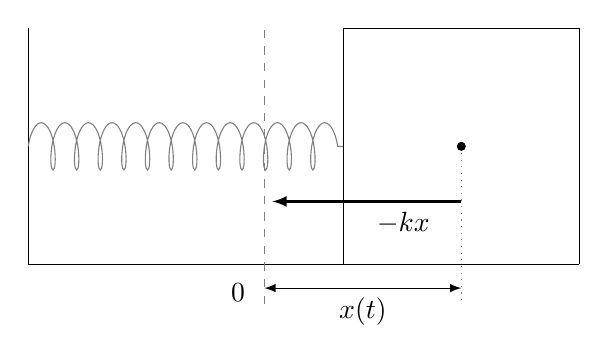
\begin{tikzpicture}
\draw[-] (0,0) -- (7,0);
\draw[-] (0,0) -- (0,3);

\draw[-] (4,0) -- (4,3) -- (7,3) -- (7,0);

\draw[gray,dashed] (3,-0.5) -- (3,3);
\draw[gray,dotted] (5.5,1.5) -- (5.5,-0.5);
\draw[thick,->] (5.5,0.8) -- node[below right, fill=white] {$-kx$} (3.1,0.8);
\node[label=below left:{$0$}] at (3,0) {};

\draw[gray,decoration={aspect=0.3, segment length=3mm, amplitude=3mm,coil},decorate] (0,1.5) -- (4,1.5);

\draw[<->] (3,-0.3) -- node[below] {$x(t)$} (5.5,-0.3);
\node[draw, fill=black, circle, inner sep=1pt] at (5.5,1.5) {};
\end{tikzpicture}
\caption{Sistema masa-resorte, con la fuerza del muelle $-kx$.}
\label{imgMasaResorte1}
\end{figure}

Según la ley de Hooke, la fuerza será

\[ F = -kx \]

donde $k$ es una constante que depende del muelle. Por lo tanto, la ecuación que describe el movimiento es 

\[ mx'' = -kx \]

Podemos transformarla a un problema en derivadas ordinarias

\begin{align*}
x'' + \frac{k}{m}x = 0
x(0) = x_0
x'(0) = v_0
\end{align*}

para el que necesitaremos posición y velocidad iniciales. 

El polinomio característico es

\[ λ^2 + \frac{k}{m} = 0 \]

cuyas raíces son 

\[ λ=\pm \i\sqrt{\frac{k}{m}} \]

Las soluciones complejas son, por lo tanto,

\begin{gather*}
z_1 = e^{\i t\sqrt{\frac{k}{m}}} = \cos \sqrt{\frac{k}{m}} t + \i \sin \sqrt{\frac{k}{m}} t \\
z_1 = e^{-\i t\sqrt{\frac{k}{m}}} = \cos \sqrt{\frac{k}{m}} t - \i \sin \sqrt{\frac{k}{m}} t 
\end{gather*}

Combinándolas de forma lineal, obtenemos dos soluciones reales:

\begin{gather*}
x_1(t) = \Re z_1 = \cos \sqrt{\frac{k}{m}} t \\
x_2(t) = \Im z_1 = \sin \sqrt{\frac{k}{m}} t
\end{gather*}

Aunque se ve a simple vista que esas dos soluciones son independientes (son coseno y seno), deberíamos calcular el wronskiano para comprobar que son realmente independientes.

La solución general nos queda

\begin{equation}\label{eqMasaResorte} x(t) = A\cos \sqrt{\frac{k}{m}} t + B \sin \sqrt{\frac{k}{m}} 
\end{equation}

Las constantes $A$ y $B$ se tendrán que obtener una vez dados los valores iniciales. Si suponemos $x(0) = x_0$, $x'(0) = v_0$, tenemos que

\begin{gather*}
x_0 = x(0) = A \\
x'(t) = -x_0 \sqrt{\frac{k}{m}} \sin \sqrt{\frac{k}{m}} t + B \sqrt{\frac{k}{m}}\cos\sqrt{\frac{k}{m}} t \\
v_0 = x'(0) = B \sqrt{\frac{k}{m}} \\
B = \frac{v_0}{\sqrt{\frac{k}{m}}}
\end{gather*}

Si bien esta solución está perfectamente bien, los físicos son gente rara y prefieren hacer otra cosa. Reescriben el punto $(A,B)$ en coordenadas polares, de tal forma que

\begin{align*}
A &= R\cos φ \\
B &= R\sin φ 
\end{align*}

Sustituyendo en \eqref{eqMasaResorte}

\[ x(t) = R\left(\cos \sqrt{\frac{k}{m}} t\cos φ + \sin \sqrt{\frac{k}{m}} t \sin φ \right) = R\cos\left(\sqrt{\frac{k}{m}}t - Φ\right) \]

donde $Φ = \arctan \frac{B}{A}$ es el desfase, que actúa de velocidad inicial del sistema.

\paragraph{Sistema masa-resorte con rozamiento}

Replanteemos el problema anterior con rozamiento.
\begin{figure}
\centering
\begin{tikzpicture}
\draw[-] (0,0) -- (7,0);
\draw[-] (0,0) -- (0,3);

\draw[-] (4,0) -- (4,3) -- (7,3) -- (7,0);

\draw[gray,dashed] (3,-0.5) -- (3,3);
\draw[gray,dotted] (5.5,1.5) -- (5.5,-0.5);
\draw[thick,->] (5.5,2) -- node[above right, fill=white] {$-εx'$} (2.7,2);
\draw[thick,->] (5.5,0.8) -- node[below right, fill=white] {$-kx$} (3.1,0.8);
\node[label=below left:{$0$}] at (3,0) {};

\draw[gray,decoration={aspect=0.3, segment length=3mm, amplitude=3mm,coil},decorate] (0,1.5) -- (4,1.5);

\draw[<->] (3,-0.3) -- node[below] {$x(t)$} (5.5,-0.3);
\node[draw, fill=black, circle, inner sep=1pt] at (5.5,1.5) {};
\end{tikzpicture}
\caption{Sistema masa-resorte con rozamiento (fuerza $-εx'$).}
\end{figure}

La ecuación cambia al añadir el rozamiento:

\begin{gather} mx'' = -kx - εx' \nonumber \\
x'' + \frac{ε}{m}x' + \frac{k}{m}x = 0
\end{gather}

Resolvemos el polinomio característico \[ λ^2 + \frac{ε}{m}λ + \frac{k}{m} = 0 \] y nos queda

\[ λ = \frac{-ε}{2m} \pm \sqrt{\left(\frac{ε}{2m}\right)^2 - \frac{k}{m}} \].

Tenemos que plantear tres casos basados en el valor de $Δ =\left(\frac{ε}{2m}\right)^2 - \frac{k}{m}$: si es mayor, igual o menor que cero.

\subparagraph{Primer caso: $Δ > 0$ (rozamiento alto)}

Tenemos 

\begin{gather*}
λ_+ = \frac{-ε}{2m} + \sqrt{\left(\frac{ε}{2m}\right)^2 - \frac{k}{m}} \\
λ_- = \frac{-ε}{2m} - \sqrt{\left(\frac{ε}{2m}\right)^2 - \frac{k}{m}} 
\end{gather*}

De sus expresiones vemos que tanto $λ_+$ como $λ_-$ son negativos. La solución general del problema es 

\( x(t) = Ae^{λ_+t} + Be^{λ_-t} \)

Despejando de los valores iniciales $x(0) = x_0$, $x'(0) = v_0$ y haciendo cuentas,

\[ x(t) = \frac{1}{λ_+ - λ_-}\left((v_0-λ_-x_0)e^{λ_+t} - (v_0-λ_+x_0)e^{λ_-t}\right) \]

De esa ecuación vemos que, cuando $t\to ∞$, $x(t) \to 0$. Es decir, el objeto tiende a pararse.

También querríamos ver cuántas veces pasamos por la posición de equilibrio. Tenemos que resolver la ecuación

\[ e^{(λ_+ - λ_-)t} = \frac{v_0-λ_+x_0}{v_0-λ_-x_0} \]

que no tiene solución. Por lo tanto, el objeto no llega nunca a la posición de equilibrio.

\subparagraph{Segundo caso: $Δ=0$}

En este caso, tenemos $λ=\frac{-ε}{2m}$ que es una raíz doble. Por el método de variación de las constantes, nuestras dos soluciones son

\[ x_1(t) = e^{\frac{-ε}{2m}t};\quad x_2(t) = te^{\frac{-ε}{2m}t} \]

y la solución general se expresa como 

\( x(t) = A e^{\frac{-ε}{2m}t} + B t e^{\frac{-ε}{2m}t} = e^{\frac{-ε}{2m}t} \left(A + Bt\right) \)

Al igual que en el anterior caso, $x(t) \convs[][t][∞] 0$, pero aquí $x(t) = 0$ sí que podemos tener soluciones.

\subparagraph{Tercer caso: $Δ < 0$ (sin rozamiento)}

Aquí tendremos raíces complejas, es decir:

\[ λ_+ = \frac{-ε}{2m} + \i \sqrt{\frac{k}{m} - \left(\frac{ε}{2m}\right)^2} \]

y su conjugada. De esta forma, las dos soluciones reales serán

\begin{gather*}
x_1(t) = e^{\frac{-ε}{2m}t} \cos t\sqrt{\frac{k}{m} - \left(\frac{ε}{2m}\right)^2} \\
x_1(t) = e^{\frac{-ε}{2m}t} \sin t\sqrt{\frac{k}{m} - \left(\frac{ε}{2m}\right)^2} \\
\end{gather*}

Podemos extraer la solución general y hacer el cambio del anterior apartado, pasando a polares $(A,B) \sim (R\cos φ, R\sin φ)$s, de tal forma que nos queda la solución general

\( x(t) = R e^{-\frac{ε}{2m}t} \cos \left(t\sqrt{\frac{k}{m} - \left(\frac{ε}{2m}\right)^2} - Φ\right) \)

Es decir, hay un decaimiento exponencial de la amplitud. La gráfica de la función sería la de la figura \ref{imgMasaResorteSeno}

\easyimg{img/MasaResorteSeno.png}{$x(t)$ para un sistema masa-resorte}{imgMasaResorteSeno}

\paragraph{Péndulo simple}

Consideramos un péndulo simple sin rozamiento.

\begin{figure}[hbtp]
\centering
\begin{tikzpicture}
\draw[-] (-2,0) -- (2,0);
\draw[-] (0,1) -- (0,-4);

\draw[-] (0,0) -- (1,-2);
\draw[->] (1,-2) -- node[right] {$mg$} (1,-3.5);
\node[draw, fill=white, circle, inner sep=4pt] at (1,-2) {};
\end{tikzpicture}
\caption{El péndulo}
\end{figure}

Tenemos las ecuaciones de posición

\[ σ(t) = (L\sin θ(t), - L \cos θ(t))\]

, de velocidad

\[ σ'(t) = (Lθ'(t)\cos θ(t), Lθ'(t)\sin θ(t))\]

y aceleración

\begin{align*}
 σ''(t) = (&-L(θ'(t))^2\sin(t) + Lθ''(t)\cos(t), \\
 & L(θ'(t))^2\cos θ(t) + Lθ''(t)\sin θ(t) 
 \end{align*}.
 
Dividimos en la componente tangencial y la perpendicular a la cuerda. Igualando algo

\[ mg( -\cosθ, -\sin θ)\sin θ  = m σ''(t) \]

y por lo tanto nos quedan las dos ecuaciones
\[ 
\left\{\begin{matrix}
 -g\sin θ \cos^2 θ = -L θ'^2 \cos θ \sin θ+ Lθ''\cos^2θ  \\
 -g\sin θ \sin^2 θ = -L θ'^2 \sin θ \cos θ  + Lθ''\sin^2θ  
 \end{matrix}\right\} \]
 
 La ecuación final es \[ -g\sin θ = L θ'' \] o, transformada 
 
 \[ θ'' + \frac{g}{L} \sin θ = 0 \]

Por Taylor, podemos aproximar $\sin θ \sim θ$ cuando θ es pequeña, de tal forma que nos reducimos al caso de un sistema masa-resorte.

\subsection{Problemas lineales no homogéneos con coeficientes constantes}

¿Qué ocurre cuando consideramos sistemas con fuerzas externas? Un ejemplo sería la siguiente ecuación en orden dos:

\(\label{eqEcOrden2} x'' + ax' + bx = f(t) \)

donde $f(t)$ representa esa fuerza externa. Tal y como habíamos visto en anteriores secciones, la solución general $X_G$ se escribía como una solución particular $X_P$ más todas las asociadas al homogéneo $X_H$. En esta situación, el problema es encontrar la solución particular, para lo cual teníamos varios métodos.

\subsubsection{Método de variación de constantes}
\label{secMetodoVarConst}
\index{Variación!de constantes} 

Siguiendo con el ejemplo en orden 2, tenemos 

\[ x_H (t) = c_1x_1(t) + c_2x_2(t) \]

y buscamos \[ x_p(t) = c_1(t)x_1(t) + c_2(t) + x_2(t) \]. Para ello derivamos:

\begin{align*}
x_p'&= c_1'x_1 + c_1x_1' + c_2'x_2 + c_2x_2' = \\
	&= c_1'x_1 + c_1 \\
x_p'' 	&= c_1''x_1+c_1'x_1' + c_2''x_2+c_2'x_2' + \\ 
		&\quad+ c_1'x_1'+c_1x_1'' + c_2'x_2' + c_2x_2'' = \\
		&= x_1''x_1 + c_2''x_2+2c_1'x_1'+2c_2'x_2' + c_1x_1'' +c_2x_2'' 
\end{align*}

Sustituyendo en \eqref{eqEcOrden2}:

\begin{align*}
f(t) &= x_p'' + ax_p' + bx_p = &  \\
	&= c_1''x_1 + c_2''x_2 + 2c_1'x_1' + 2c_2'x_2'  + c_1x_1''  + c_2x_2'' \\
	& + ac_1' x_1 + ac_2'x_2  + ac_1x_1'  + ac_2x_2' \\
	&  + bc_1x_1  + bc_2x_2 
\end{align*}

Hemos acabado con un enorme caos de variables y cosas. Sin embargo, recordamos que no buscamos todos las soluciones, sino que sólo nos basta con una. Planteamos 

\[ c_1'x_1 + c_2'x_2 = 0 \] y \[ c_1'x_1' + c_2'x_2' = f \]
 
Que nos lleva a un sistema

\[ \underbrace{\begin{pmatrix}
x_1 & x_2 \\
x_1' & x_2' 
\end{pmatrix}}_A\begin{pmatrix}
c_1' \\ c_2'
\end{pmatrix} = \begin{pmatrix}
0 \\ f(t)
\end{pmatrix} \] 

que tiene solución, ya que al ser $x_1,x_2$ soluciones independientes, el wronskiano (igual al determinante de $A$ es distinto de $0$).

En un caso general de orden $n$, el sistema a plantear será

\[ \begin{pmatrix}
x_1 & \cdots & x_n \\
x_1' & \cdots & x_n \\
\vdots & \ddots & \vdots \\
x_1^{n)} & \cdots & x_n^{n)}
\end{pmatrix} \begin{pmatrix} c_1' \\ c_2' \\ \vdots \\ c_n' \end{pmatrix} 
= 
\begin{pmatrix}
0 \\ \vdots \\ 0 \\ f(t)
\end{pmatrix} \]

Apliquemos ahora este desarrollo a algún ejemplo.

\paragraph{Ejemplo} $x'' + x = e^t$

Buscamos $x_p(t) = c_1(t) x_1 + c_2(t) x_2$, donde

\[ \underbrace{\begin{pmatrix}
x_1 & x_2 \\
x_1' & x_2' 
\end{pmatrix}}_A\begin{pmatrix}
c_1' \\ c_2'
\end{pmatrix} = \begin{pmatrix}
0 \\ e^t
\end{pmatrix} \] 

Podemos elegir $x_1$ y $x_2$ como seno y coseno:

\[ \underbrace{\begin{pmatrix}
\cos t & \sin t \\
- \sin t & \cos t 
\end{pmatrix}}_A\begin{pmatrix}
c_1' \\ c_2'
\end{pmatrix} = \begin{pmatrix}
0 \\ e^t
\end{pmatrix} \] 

y resolvemos el sistema. Nos queda que 

\[ c_2' = e^t \cos t \]

y haciendo cuentas desagradables sale. Sin embargo, a ojo vemos que una solución particular es

\[ x_p(t) = \frac{e^t}{2} \]

¿Qué tiene de especial este problema? Esa exponencial en $f(t)$. Esto nos lleva a otro método, el de coeficientes indeterminados.

\subsubsection{Método de coeficientes indeterminados}

Podremos aplicar este método cuando $f(t)$ sea un polinomio, una exponencial, senos y cosenos y combinaciones lineales de todos los anteriores. En todos estos casos las derivadas nos llevan a funciones de la misma clase, y podremos aplicar este método que nos lleva a cuentas más sencillas.

En este método, suponemos que la solución particular es una función de la misma familia de $f(t)$ multiplicada por una constante, así que planteamos el problema y resolvemos el sistema. Estudiémoslo desde un ejemplo:

\paragraph{1)} \[ x'' - x = e^{2t} \]

Tenemos que 
\begin{gather*}
x_p(t) = Ce^{2t} \\
x_p' = 2Ce^{2t} \\
x_p'' = 4Ce^{2t} \\
e^2t = 4Ce^{2t} - Ce^{2t} = 3Ce^{2t} 
\end{gather*}

$C$ ha de ser $\frac{1}{3}$ y por lo tanto nuestra solución general del sistema será

\[ x_G = c_1e^t + c_2e^{-t} + \frac{1}{3}e^{2t} \]

\paragraph{2)} Otro ejemplo:

\[ x''-x= e^t \]

Aquí habría que calcular $x_p = ce^t$. Sin embargo, nos quedaría $x_p'' - x_p = 0 ∀c$. Cuando $f(t)$ es una de las soluciones de la ecuación homogénea asociada, tenemos que añadir algo más. Buscamos soluciones de la forma $cte^t$

\begin{gather*}
x_p  = cte^t \\
x_p' = cte^t + ce^t \\
x_p'' = cte^t + 2ce^t \\
\end{gather*}

Resolviendo:

\begin{align*}
x_p'' - c_p &= 2ce^t \\
e^t &= 2ce^t \\
C &= \frac{1}{2} 
\end{align*}

\paragraph{3)} Probamos ahora con senos y cosenos.

\[ x'' + x= \cos 2t\]

En este caso, la solución debe tener una combinación lineal de senos y cosenos. Por lo tanto

\[ x_p = A\cos 2t + B\sin 2t \]

y resolviendo

\[ \cos 2t = x_p'' + x_p = -3A\cos 2t - 3B\sin 2t \]

de tal forma que $A=\frac{-1}{3}$ y $B=0$.

\paragraph{4)} Consideramos $x''+x = \cos t$. 

En este caso, $f(t) = \cos t$ es una solución de la parte homogénea, así que la solución será de la forma

\[ x_p(t) = At\cos t + Bt\sin t \]

Supongamos que esto modela una situación real, como por ejemplo empujando un columpio. ¿Cómo interpretamos esto? 

A ciertas frecuencias, la ecuación es creciente, la amplitud aumenta con el tiempo. Es un fenómeno de \textbf{resonancia}. Veamos cómo modelizar este caso.

\paragraph{Ejemplo: Sistema masa-resorte con fuerza externa}

La ecuación en este caso es

\(\label{eqMRF1} x'' + \underbrace{\frac{k}{m}}_{=ω^2}x = \underbrace{f(t)}_{F\cos αt} \)

Hemos cambiado algunas constantes para adaptarlo a nuestro caso. Hay varias opciones a partir de aquí relacionadas con las constantes ω y α:

\subparagraph{Caso 1: $ω≠α$}

Resolvemos la ecuación homogénea $x''+ω^2 x = 0$ con el polinomio característico:

\[ λ^2+ω^2  = 0 \implies λ = \pm ω\i \]

y por lo tanto

\( x_H(t) = c_1 \cos ωt + c_2 \sin ωt \)

Necesitamos ahora una solución particular $x_P = A\cos αt + B\sin αt$. Derivamos dos veces:

\begin{gather*}
x_P(t) = A\cos αt + B\sin αt \\
x_P'(t) = -Aα\sin αt + Bα\cos αt \\
x_P''(t) = -Aα^2\cos αt - Bα^2\sin αt 
\end{gather*}

Sustituyendo en \eqref{eqMRF1}

\begin{gather*}
 F\cos αt = x_P'' + ω^2x_P = \dotsb = (ω^2-α^2)\left(A\cos αt + B\sin αt\right) \\
 B = 0;\quad A= \frac{F}{ω^2-α^2} \\
 x_P(t) = \frac{F}{ω^2-α^2}\cos αt
\end{gather*}

De esta forma, la ecuación general nos queda

\( x_G(t) = \frac{F}{ω^2-α^2}\cos αt + c_1 \cos ωt + c_2 \sin ωt \)

Para los datos iniciales $x(0) = x'(0) = 0$, despejamos y tenemos la solución al problema

\(\label{eqMRF2-Sol} x(t) = \frac{F}{ω^2-α^2}\left(\cos αt - \cos ωt\right) \)

Volviendo de nuevo al sistema que tratamos, ω y α representan dos frecuencias. α es la externa y ω es la natural. Podemos reescribir la ecuación \eqref{eqMRF2-Sol} usando identidades trigonométricas. Sabemos que

\[ \cos (A-B) - \cos(A+B) = 2\sin A \sin B \]

Resolvemos:

\[ \left.\begin{matrix}A - B = αt \\ A + B = ωt \end{matrix}\right\}
\left.\begin{matrix}A = \frac{ω+α}{2}t \\ B = \frac{ω-α}{2}t\end{matrix}\right\} \]

Sustituyendo en \eqref{eqMRF2-Sol}:

\( x(t) = \frac{2F}{ω^2-α^2} ·\sin \frac{ω-α}{2}t · \sin \frac{ω+α}{2}t  \)

Luego lo que tenemos es una oscilación rápida (Δ) con una amplitud contenida dentro de otra con oscilación más lenta (Γ).

\easyimg{img/MasaResorteF.png}{Gráfico de una oscilación rápida (Δ, azul) con una amplitud contenida dentro de otra con oscilación más lenta (Γ, verde)}{imgMasaResorteF}

\subparagraph{Caso 2: $ω=α$}

En este caso, la ecuación diferencial es 

\[ x'' + ω^2 x = F\cos ωt \]

La solución de la homogénea es $x_H = c_1 \cos ωt + c_2 \sin ωt$. Tenemos un problema: $F\cos ωt$ es solución de la homogénea. Para encontrar una solución particular multiplicamos entonces por $t$:

\begin{gather*}
x_P = t\left(A\cos ωt + B\sin ωt\right) \\
x_P' =t\left(-Aω\sin ωt + Bω\cos ωt\right) + \left(A\cos ωt + B\sin ωt\right) \\
x_P'' = t\left(-Aω^2 \cos ωt - Bω^2 \sin ωt\right) + 2\left(-Aω\sin ωt + Bω\cos ωt \right)
\end{gather*}

Igualando, 

\[ F\cos ωt \qeq x_p'' + ω^2x_p = 2\left(-Aω\sin ωt + Bω\cos ωt \right) \]

de donde sacamos que $A=0$ y $B=\frac{F}{2ω}$. Una solución particular es entonces

\[ x_P(t) = \frac{F}{2ω}t \sin ωt \]

que es además la solución que cumple $x_P(0) = x_P'(0) = 0$. La gráfica de esta ecuación será

\easyimg{img/MasaResorteF-Resonancia.png}{Gráfica de un sistema masa-resorte en resonancia}{imgMasaResorteFR}

Estamos ante un fenómeno de resonancia. La amplitud tiene a infinito siempre, por muy pequeña que sea la fuerza.

Que, por cierto, Azorero nos ha engañado en una cosa: la expresión de la fuerza es un coseno en lugar de una función genérica $F(t)$. En realidad esto se debe al desarrollo en serie de Fourier, que dice que cualquier función se puede expresar como 

\[ F(t) = \sum_{j=0}^∞ F_j \cos \frac{jπ}{T}t \]

\paragraph{Modelo con rozamiento}

Añadiendo el rozamiento al modelo anterior, tenemos

\[ x''+2εx'+ω^2x = \cos αt \]

Haciendo cuentas y suponiendo $ε^2-ω^2<0$. Nos queda una solución para la homogénea

\[ x_H = e^{-εt}\left(c_1 \cos \sqrt{ω^2-ε^2}t + c_2 \sin \sqrt{ω^2-ε^2}t\right) \]

Buscamos la solución particular

\[ x_P (t) = A\cos αt + B\sin αt \]

y llegamos a 

\[ x_P(t) = \frac{1}{(ω^2-α^2)^2 + 4α^2ε^2}\left((ω^2-α^2)\cos αt + 2αε \sin αt \right) \].

La solución general es entonces

\[ x_G(t) = x_P(t) + x_H(t) \]

Dado que en $x_H$ está todo multiplicado por una exponencial negativa, tiende a cero cuando $t\to ∞$, por lo que la llamamos la parte \textbf{transitoria}. El primer sumando, $x_P$, permanece y se le llama la parte \textbf{estacionaria}.

En este caso, cuando $α=ω$ (estamos en la frecuencia de resonancia), es el que más aporta a la ecuación. Sin embargo, en ningún caso la amplitud se va a infinito. El rozamiento impide que la amplitud se dispare.

\subsubsection{Resumen de métodos para ec. lineales no homogéneas}

Hagamos un resumen de los métodos que hemos visto. Las soluciones de una ecuación no homogénea de la forma

\[ y^{n)} + a_{n-1}y^{n-1)} + \dotsb + a_1y'+a_0y = f(t) \]

se expresan en función de una solución particular $y_p$ y el conjunto de las soluciones para la ecuación homogénea asociada $y_H$:

\[ y_G = y_p + y_H \]

Podemos obtener fácilmente las soluciones a la homogénea usando la técnica vista en la sección anterior \eqref{secEcHomoLinealConstante}. Para obtener la solución particular tenemos que usar el método de variación de constantes (\ref{secMetodoVarConst}). Sin embargo, ese método nos lleva a muchas más cuentas de las necesarias. Podemos simplificar las cosas cuando $f(t)$ pertenece a una familia de curvas "cerrada" por la derivada. Veamos esos casos.

\paragraph{Polinomio}

\[ f(t) = A_0 + A_1t + \dotsb + A_Nt^N \]

Si $0$ no es raíz, buscamos \[y_p(t) = a_0 + a_1t + \dotsb + a_Nt^N\]. Si $0$ es raíz con multiplicidad $k$, entonces la solución particular que buscamos será de la forma

\[ y_p(t) =( a_0 + a_1t + \dotsb + a_Nt^N)t^k \]

\paragraph{Trigonométrico} 

\[ f(t) = \cos αt \]

o análogamente para senos. Tenemos dos posibilidades. Si $α\i$ no es raíz del p. característico, la solución particular es de la forma

\[ y_p(t) = a\cos αt + b\sin αt \]

En el caso de que $α\imath$ sea raíz con multiplicidad $k$, entonces

\[ y_p(t) = (a\cos αt + b\sin αt)t^k \]

\paragraph{Polinomio y exponencial}

\[ f(t) = e^{αt}(A_0 + A_1t + \dotsb + A_Nt^N) \]

Si $α$ no es raíz del p. característico,

\[ y_p(t) = e^{αt}(a_0 + a_1t + \dotsb + a_Nt^N) \]. si α sí es raíz con multiplicidad $k$,

\[ y_p(t) = t^ke^{αt}(a_0 + a_1t + \dotsb + a_Nt^N) \]

\subsection{Ejemplos}

\begin{example} Consideramos la ecuación

\[ y'' + a' + by = 0 \]

Demuestra que 

\[ y_H(t) \convs[][t][∞] \iff a>0, b>0 \]

Empezamos por la implicación a la izquierda. El polinomio característico es

\[ λ^2+aλ+b \implies λ_{\pm} = \pm \frac{a\pm \sqrt{a^2-4b}}{2} \]

Tenemos tres casos:

\begin{itemize}
\item $a^2-4b > 0$. En este caso, $λ_-,λ_+ ∈ℝ$, $λ_-<λ_+<0$ y por lo tanto $e^{λ_+t}$ y $e^{λ_-t}$ tienden a cero cuando $t\to ∞$.

\item $a^2=4b$. Aquí tenemos que $λ=\frac{-a}{2}$, raíz doble. Las soluciones son $e^{\frac{-a}{2}t}$ y $te^{\frac{-a}{2}t}$, ambas tienden a cero.

\item $a^2-4b > 0$. Las raíces son imaginarias y te sale igual porque lo ha borrado.

\end{itemize}

Para demostrar la implicación a la derecha, tenemos que si $y_H(t)\convs[][t][∞]0$, entonces los autovalores del p.c. son o bien

\[ y_\pm = α\pm + \iβ \]

con $α<0$ o bien reales con $λ_-≤λ_+<0$. En ambos casos tenemos que $a>0, b>0$ tal y como hemos visto al demostrar la otra implicación.

\end{example}

\begin{example}[Ejercicio 7]

Tenemos la siguiente ecuación:

\[ y^{iv)} + 4y''' + 8y'' + 8y' +4y = 0\]

y nos dicen que $\i - 1$ es raíz del p.c.

\[ P(λ) = λ^4 + 4λ^3 + 8λ^2 + 8λ + 4 = 0 \]

Sabiendo que $\i-1$ es raíz y que su conjugado $-\i - 1$ también, podemos hacer las cuentas y

\begin{gather*}
 P(λ) = (λ-(-1+\i)) · (λ-(-1-\i)) · P_2(λ) \\
 ((λ+1)^2 + 1) P_2(λ)
 \end{gather*}

donde 

\[ P_2(λ) = \frac{λ^4+ 4λ^3 + 8λ^2 + 8λ + 4 }{λ^2+2λ + 2} = \dotsb = λ^2 + 2λ + 2 \].

Por lo tanto las dos raíces son dobles.
\end{example}

\begin{example}[Ejercicio 8] Tenemos la ecuación

\[ y^{n)} + a_{n-1}y^{n-1)} + \dotsb + a_1y' + a_0y = x^k \]

con $a_0≠0$. Demostrar que en el caso $n=4,k=3$, existe un único polinomio que sea solución del problema, que además tiene grado 3.

Hay que demostrar dos cosas: que existe y que es único. Empezamos demostando la unicidad suponiendo que existen $P,Q$ polinomios de grado tres solución.

En este caso tendríamos que $P-Q$ es solución de la homogénea. Y ha dicho algo y no lo he podido copiar.

Demostramos ahora la existencia. Buscamos una solución polinómica $y(x) = c_0+c_1x + c_2x^2 + c_3x^3$. Si calculamos

\[ a_0y(x) + a_1y'(x) + a_2y''(x) + a_3y'''(x) = x^3 = \underbrace{\{c_j,a_j\}}_{=0} + \underbrace{\{c_j,a_j\}x}_{=0} + \underbrace{\{c_j,a_j\}x^2}_{=0} + \underbrace{\{c_j,a_j\}}_{=1}x^3 \]

donde $\{c_j,a_j\}$ son combinaciones lineales de cada una de las $a_j$ y $c_j$. Tendremos entonces un sistema con coeficientes $a_j$ e incógnitas $c_j$ de la forma

\[ A \begin{pmatrix}
c_0 \\ c_1 \\ c_2 \\ c_3
\end{pmatrix} = \begin{pmatrix}
0 \\ 0 \\ 0 \\ 1
\end{pmatrix} \]
\end{example}

\begin{example}[Ejercicio 11]

Tenemos la ecuación

\[ y'' + P(t) y' + Q(t) y = 0 \]

Decir sobre qué condiciones de $P,Q$ el cambio de variables $s=Φ(t), z(s) = y(t)$ convierte la ecuación en una coeficientes constantes. 

Calculamos las derivadas:

\begin{gather*}
 \od{y}{t} = \od{y}{t} \od{s}{t} = \od{z}{s} \od{Φ}{t} \\
 \od[2]{y}{t} = \od[2]{z}{s} \left(\od{Φ}{t}\right)^2 + \od{z}{s}\od[2]{Φ}{t}
\end{gather*}

y sustituyendo

\[ 0 = \od[2]{z}{s} + \underbrace{\left(\frac{\od[2]{Φ}{t} + P\od{Φ}{t}}{\left(\od{Φ}{t}\right)^2}\right)}_{A} \od{z}{s} + \underbrace{\frac{Q}{\left(\od{Φ}{t}\right)^2}}_{B}z \]

tenemos que buscar las condiciones sobre $P$ y $Q$ y la expresión de $Φ(t)$ para que ahí haya constantes multiplicando a $\od{z}{s}$ y a $z$. Entonces

\[ \frac{Q}{\left(\od{Φ}{t}\right)^2} = B \implies \left(\od{Φ}{t}\right)^2 = \frac{Q}{B} \implies \od{Φ}{t} = \sqrt{\frac{Q}{B}} \]

Sustituyendo:

\[ A = \frac{\od[2]{Φ}{t} + P\sqrt{\frac{Q}{B}}}{\left(\od{Φ}{t}\right)^2} \]

Casi tenemos la relación, pero tenemos que deshacernos de esa segunda derivada. Así que derivamos:

\[ \od[2]{Φ}{t} = \frac{-A}{2\sqrt{B}\sqrt{Q}}Q' \]

y sustituimos 

\[ A = \frac{\frac{-A}{2\sqrt{B}\sqrt{Q}}Q' + P\sqrt{\frac{Q}{B}}}{\left(\od{Φ}{t}\right)^2} = \dotsb = \frac{Q'+2PQ}{Q\sqrt{Q}} = \text{cte.} \]

y además tiene que ser

\[ (Φ'(t))^2 = \frac{Q(t)}{B} \]

\end{example}

\section{Teoremas de existencia y unicidad}

Partiendo del problema

\[ \begin{cases}
y' = f(x,y(x)) \\
y(x_0) = y_0
\end{cases} \]

podemos hacer una \textbf{formulación integral equivalente} de la forma

\[ y(x) = y_0 + \int_{x_0}^x f(s,y(s))\dif s \].

Hay dos posibles aproximaciones para resolver este problema.

\paragraph{Iteradas de Picard}\index{Iteradas!de Picard} Veamos este método con un ejemplo. Partimos de 

\[ \begin{cases}
y' = y \\
y(x_0) = 1
\end{cases} \].

La primera aproximación será

\[ y_1(x) = 1 + \int_0^x y_0 \dif x = 1+ \int_0^x 1\dif s = 1 + x \]. Hacemos una segunda aproximación:

\[ y_2(x) = 1 + \int_0^x y_1 \dif x = 1 + \int_0^x 1+s \dif s  = 1 + x +\frac{x^2}{2} \]

Podríamos seguir haciendo iteradas basándonos en la misma fórmula

\(\label{eqIteradasPicard} y_n(x) = 1 + \int_0^x y_{n-1}(s) \dif s \)

y veríamos que lo que sale es el polinomio de Taylor de la exponencial. Planteamos entonces un algoritmo iterativo siguiendo la ecuación \eqref{eqIteradasPicard}. Si consiguiésemos demostrar que

\begin{itemize}
\item $y_n(x) \convs[][n] y(x)$.
\item $\displaystyle\lim_{n\to\infty} \int_{x_0}^x f(s,y_{n-1}(s))\dif s = \int_{x_0}^x \lim_{n\to ∞} f(s,y_{n-1}(s)) \dif s$.
\item $\displaystyle\lim_{n\to ∞} f(s, y_{n-1}(s)) = f(s,y(s))$.
\end{itemize}

tendríamos siempre una solución al problema. Sin embargo, no es trivial definir qué es un límite de funciones, entrando dentro del análisis funcional. Además, deberíamos ver hasta qué $x$ podríamos usar la solución. 

Buscamos por lo tanto otro método para resolver el problema.

\paragraph{Método de las poligonales de Euler}\index{Poligonales!de Euler} Supongamos que la solución exacta del problema es $y(x)$. Entonces, para un $x_1=x_0 + h$, podemos decir que

\[ y(x_1) = y(x_0 + h) \stackrel{\text{Taylor}}{=} y(x_0) + y'(x_0)\cdot h + \mop{error}(h) \]

Ahora bien, sabemos que $y(x_0) = y_0$ y que $y'(x_0) =f(x_0, y_0)$. Entonces

\[ y(x_1) ≈ y_0 + f(x_0, y_0)·h \equiv y_1 \]

es un valor aproximado de la solución en $x_1$. Repetimos el proceso. Tomamos $x_2 = x_1 + h$, y 

\[ y(x_2) ≈ y_1 + f(x_1,x_1)· h \equiv y_2 \]

Rehaciendo el proceso, llegamos a una poligonal $P_n$ (poligonal de Euler) que aproximará la curva:

\begin{figure}[hbtp]
\centering
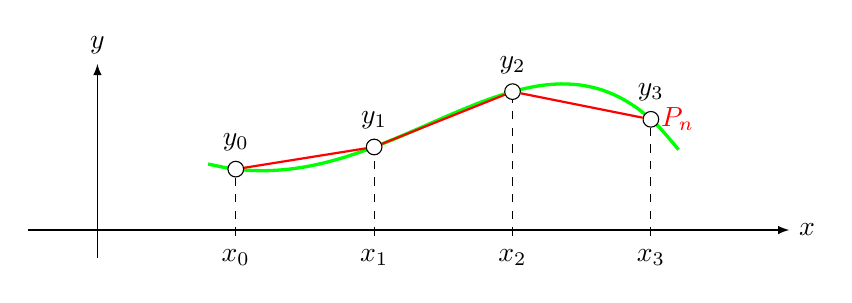
\begin{tikzpicture}[x=50pt,y=20pt]
	\draw[->] (-0.5,0) -- (5,0) node[right] {$x$};
	\draw[->] (0,-0.5) -- (0,3) node[above] {$y$};
	
	\draw[very thick,domain=0.8:4.2,smooth,variable=\x,green] plot ({\x},{2.19805 - 1.84594*\x + 0.64716*\x*\x + 0.150811*\x*\x*\x - 0.0500811*\x*\x*\x*\x});
	
	\node[draw,label=above:{$y_0$},circle, fill=white, inner sep=2pt] (A) at (1,1.1) {};
	\node[draw,label=above:{$y_1$},circle, fill=white, inner sep=2pt] (B) at (2,1.5) {};
	\node[draw,label=above:{$y_2$},circle, fill=white,inner sep=2pt] (C) at (3,2.5) {};
	\node[draw,label=above:{$y_3$},circle, fill=white, inner sep=2pt] (D) at (4,2) {};
	
	\node[label=below:{$x_0$}] at (1,0) {};
	\node[label=below:{$x_1$}] at (2,0) {};
	\node[label=below:{$x_2$}] at (3,0) {};
	\node[label=below:{$x_3$}] at (4,0) {};
	
	\draw[-, dashed] (1,-0.1) -- (A);	
	\draw[-, dashed] (2,-0.1) -- (B);
	\draw[-, dashed] (3,-0.1) -- (C);
	\draw[-, dashed] (4,-0.1) -- (D);
	
	\draw[-,thick,red] (A) -- (B) -- (C) -- (D) node[right] {$P_n$};
	
\end{tikzpicture}
\end{figure}


Entonces, deberíamos tener que

\[ y(x) \equiv \lim_{h\to 0} P_n(x) \]

Es también una solución razonable, pero llegamos a la misma dificultad que antes: no sabemos en qué consiste el límite de una sucesión de funciones.

\subsection{Análisis funcional y sucesiones de funciones}

De cualquiera de las formas tenemos que entrar en análisis funcional, así que tratemos de dar sentido a ese concepto de sucesiones de funciones. Partimos de un conjunto de funciones $\{f_n(x)\}_{n∈ℕ}$ definidas para $x∈(a,b)$. ¿Qué significa entonces el límite $\displaystyle\lim_{n\to ∞} f_n(x) = f(x)$?

Hay varias definiciones para ese límite. La primera es la convergencia puntual:

\subsubsection{Convergencia puntual}

La convergencia puntual consiste en la convergencia de cada uno de los puntos del intervalo. Es decir

\[ f_n\to f \iff \lim_{n\to ∞} f_n(x) = f(x) ∀x ∈ (a,b) \]

O, en términos de ε y δ, que para $x∈(a,b)$

\[ ∀ε>0\, ∃n_0 \tq n> n_0 \implies \abs{f_n(x) - f(x)} < ε \]

Ahora bien, hay que leer con cuidado. En esta definición, tenemos que $n_0 = n_0(ε,x)$ depende de dos parámetros. Esta definición es por lo tanto muy débil como para usarla en los métodos de resolución anteriores.
\end{document}
